\documentclass{beamer}

\usepackage{hyperref}
\usepackage{listings}
\usepackage{color}

\usepackage[backend=bibtex]{biblatex}
\addbibresource{citations.bib}

% http://tex.stackexchange.com/questions/68080/beamer-bibliography-icon
\setbeamertemplate{bibliography item}{%
  \ifboolexpr{ test {\ifentrytype{book}} or test {\ifentrytype{mvbook}}
    or test {\ifentrytype{collection}} or test {\ifentrytype{mvcollection}}
    or test {\ifentrytype{reference}} or test {\ifentrytype{mvreference}} }
    {\setbeamertemplate{bibliography item}[book]}
    {\ifentrytype{online}
       {\setbeamertemplate{bibliography item}[online]}
       {\setbeamertemplate{bibliography item}[article]}}%
  \usebeamertemplate{bibliography item}}

\defbibenvironment{bibliography}
  {\list{}
     {\settowidth{\labelwidth}{\usebeamertemplate{bibliography item}}%
      \setlength{\leftmargin}{\labelwidth}%
      \setlength{\labelsep}{\biblabelsep}%
      \addtolength{\leftmargin}{\labelsep}%
      \setlength{\itemsep}{\bibitemsep}%
      \setlength{\parsep}{\bibparsep}}}
  {\endlist}
  {\item}

% Colours for beamer.
\setbeamercolor{frametitle}{fg=orange}
\setbeamertemplate{itemize item}{\color{orange}$\blacksquare$}
\setbeamertemplate{itemize subitem}{\color{orange}$\blacktriangleright$}

% Colours for syntax highlighting
\definecolor{syntax_red}{rgb}{0.7, 0.0, 0.0} % For strings
\definecolor{syntax_green}{rgb}{0.15, 0.5, 0.25} % For comments
\definecolor{syntax_orange}{rgb}{0.7, 0.4, 0.2} % For keywords


% Haskell settings for lstlisting
\lstset{language=Haskell,
basicstyle=\ttfamily\tiny,
keywordstyle=\color{syntax_orange}\bfseries,
stringstyle=\color{syntax_red},
commentstyle=\color{syntax_green},
numbers=none,
numberstyle=\color{black},
stepnumber=1,
frame=single,
breaklines=true,
numbersep=10pt,
tabsize=4,
showspaces=false,
showstringspaces=false}

\author{
  Beck, Calvin \and Huang, Jiani \and Li, Yishuai
}

\begin{document}

\begin{frame}
  \frametitle{FuzzChick}
  \maketitle
\end{frame}

\section{Introduction}

\begin{frame}
  \frametitle{What is this talk about?}

  \pause

  {\huge FuzzChick!}\\~\\

  \pause

  What is FuzzChick...? \\~\\

  \pause

  FuzzChick is an experiment to improve QuickChick using ideas from
  fuzzing. This combines QuickChick with AFL \cite{AFL}.\\~\\~\\

  \pause

  {\huge We'll come back to this...}\\

\end{frame}

\begin{frame}
  \frametitle{QuickChick: A Brief Review}

  QuickChick is a properties based testing framework for Coq. \\

  \begin{itemize}
  \item You build (or derive) generators for data types.
  \item Using those generators you can feed data into test cases.
  \item These test cases can be any arbitrary predicate.
  \end{itemize}
\end{frame}

\begin{frame}
  \frametitle{QuickChick: Pros and Cons}

  So what's great about QuickChick?\\

  \begin{itemize}
  \item Relatively easy to build / derive generators.
  \item Can generate lots of tests for specific properties
    automatically.
  \end{itemize}

  \pause

  What's not so great about QuickChick?\\

  \pause

  \begin{itemize}
  \item Getting \emph{good} generators can be hard!
  \end{itemize}
\end{frame}

\section{Good Generators}

\begin{frame}
  \frametitle{What makes a good generator?}

  The basic idea of what makes a generator ``good'' can vary somewhat
  based on the context. \\

  \pause

  In general you want good coverage. How can you achieve that with
  minimal work?
\end{frame}

\section{FuzzChick}

\begin{frame}
  \frametitle{Finally, FuzzChick!}

  FuzzChick uses AFL to make the choices between constructors for
  building data types for tests.\\

  \pause

  Why is this good?

\end{frame}

\begin{frame}
  \frametitle{FuzzChick Intuition}

  AFL uses DSE to attempt to get good coverage while fuzzing...\\

  \pause

  Maybe we can utilize AFL's smarts to achieve better test coverage.
\end{frame}

\section{Evaluating FuzzChick}

\subsection{FuzzChick and Apache}

\subsection{FuzzChick Coverage}

\begin{frame}
  \frametitle{QuickChick: Now With Coverage!}

  We instrumented QuickChick using bisect\_ppx to get coverage
  estimates!\\~\\

  \pause

  This \emph{mostly} went smoothly...\\~\\

  
\includegraphics[width=\textwidth]{bisectbug.png} \\

  \pause

  Maintainer fixed this issue promptly, which was \emph{awesome}!
  
\end{frame}

\begin{frame}
  \frametitle{QuickChick with coverage... Still needs some polish}

  QuickChick with coverage is cool, but it still does need some
  polish.\\

  \begin{itemize}
    \pause
  \item Includes a lot of excessive extracted Coq code.
    \pause
    \begin{itemize}
    \item Like... All of QuickChick :(.
    \item So, the percentages are a little off.
    \end{itemize}
    \pause
  \item QuickChick generates ``random'' files for each test, and the
    names aren't all that useful
    \begin{itemize}
    \item Modified QuickChick to include test case in name, but still
      not ideal.
    \end{itemize}
  \end{itemize}

  \pause

  But...\\~\\

  \pause

  {\huge It works! We can measure stuff!}
\end{frame}

\begin{frame}
  \frametitle{QuickChick Coverage: ifc-basic}

  Coverage with QuickChick in the ifc-basic example: \\~\\

  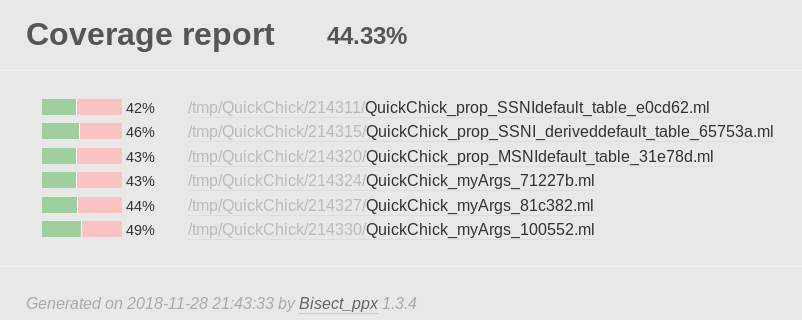
\includegraphics[width=\textwidth]{ifccoverage.png} \\
  
\end{frame}

\begin{frame}
  \frametitle{QuickChick vs FuzzChick: ifc-basic}

  QuickChick: \\~\\

  
\includegraphics[width=\textwidth]{ifcquickchick.png} \\~\\

  \pause

  FuzzChick: \\~\\

  
\includegraphics[width=\textwidth]{ifcfuzzchick.png} \\~\\
  
  For some reason it seems that FuzzChick actually gets worse coverage
  than QuickChick on this test case... At least in the time I let it run (I'm not
  terribly patient)
\end{frame}

\begin{frame}
  \frametitle{Why Worse Coverage?}

  \begin{itemize}
  \item Just need to let it run longer?
    \begin{itemize}
    \item AFL needs a while to ``warm up''?
    \end{itemize}
    \pause
  \item QuickChick test already managed to get good coverage in this
    instance, so fuzzing doesn't give us much on top of it?
    \begin{itemize}
    \item Hard to tell what ``good coverage'' is due to the extraneous
      code extracted by QuickChick.
    \end{itemize}
    \pause
  \item Something's not instrumented correctly?
    \pause
  \item This test case, for whatever reason, is fuzzer unfriendly?
    \begin{itemize}
    \item Maybe extracted Coq could be fuzzer unfriendly? Lots of
      inefficient data types like like \texttt{nat} (basically a
      linked list whose length represents a number).
    \item Could result in excessively long paths and hard to solve
      predicates for DSE?
    \item Not sure that having pointers everywhere would be AFL's
      strength...
    \end{itemize}
  \end{itemize}
\end{frame}

\begin{frame}[fragile]
  \frametitle{Some Further Coverage Testing...}

  Test case:

\begin{lstlisting}[language=Haskell]
Extract Constant unlikely_branch =>
" fun i ->
  if (0 < i)
  then if (i mod 100 == 0)
       then if (i mod 1000 == 0)
            then if (i mod 10000 == 0)
                 then if (i mod 100000 == 0)
                      then if (i mod 1000000 == 0)
                           then if (i < 1000001)
                                then 42
                                else 0
                           else 0
                      else 0
                 else 0
            else 0
       else 0
  else 0
".


Definition always_zero := forAll (choose (0%Z, 9999999%Z)) (fun n => unlikely_branch n =? 0).
\end{lstlisting}

  \pause

  {\large Trying to give AFL a good chance to find the failing branch...}

\end{frame}

\begin{frame}
  \frametitle{Results}

  In the equivalent C code AFL does quite well... \\~\\

  \pause

  QuickChick: \\

  
\includegraphics[width=\textwidth]{qc_branches.png} \\~\\

  FuzzChick: \\

  
\includegraphics[width=\textwidth]{fuzz_branches.png} \\~\\

  \pause
  
  Here not so much? FuzzChick doesn't make it as far... \\~\\

  \pause

  Well, in fairness, it does eventually, but it takes a good 30
  minutes. QuickChick was much faster. \\~\\

  \pause

  Suggests maybe the extracted ocaml is harder for AFL to analyze? The
  C branches were discovered very quickly by AFL.
  
\end{frame}

\begin{frame}
  \frametitle{Performance}
  \begin{itemize}
  \item Fuzzing is an order of magnitude slower than random testing.
  \item Performance bottleneck: disk access.
  \item Experiments to see whether the instrumentation overhead is worth it are
    still in preliminary stages.
  \end{itemize}
\end{frame}

\section{Honourable Mentions}

\begin{frame}
  \frametitle{Honourable Mentions: Some Other Stuff We Did}

  \begin{itemize}
    \pause
  \item Honggfuzz!
    \pause
    \begin{itemize}
    \item Finally got this working...
    \item Didn't really work out because it takes a long time to find
      bugs by fuzzing.
    \item Decided it wasn't really a great comparison to FuzzChick
      which is a properties based testing tool anyway.
    \item Some useful scripts / documentation to get this running in
      our git repo. \cite{quick700}
    \end{itemize}
    \pause
  \item Plain AFL!
    \pause
    \begin{itemize}
    \item Similar story to Honggfuzz.
    \end{itemize}
  \end{itemize}
\end{frame}

\section{End}

\begin{frame}
  \frametitle{Conclusion! Questions?}

  \huge{Whew! Questions?}
\end{frame}

\begin{frame}
  \frametitle{References}

  \nocite{*}
  \printbibliography

  These are all good resources! You should look at them!
\end{frame}
\end{document}
